\section{Zielsetzung}
\label{sec:Zielsetzung}
Das Ziel des Versuchs ist die Auseinandersetzung mit dem Photoeffekt. 
Dazu wird die Strom-Spannungskennlinie einer Photozelle gemessen und 
das Plancksche Wirkungsquantum bestimmt. 
\section{Theorie}
\label{sec:Theorie}
Grundlegend für den Versuch ist der Lichtelektrische Effekt. Dieser 
beschreibt das Auslösen von Elektronen aus einem Metall durch Licht. 
Dieser kann außerdem dazu verwendet werden das Plancksche Wirkungsquantum $h$
zu bestimmen. Notwendig dafür ist die Relation 
\begin{equation}
    E_\gamma = h \cdot \nu
\end{equation}
$E_\gamma$ ist Strahlungsenergie eines Photons und $\nu$ ist die Frequenz 
des Photons. Wird ein Metall mit Licht bestrahlt, kann die Energie 
eines Lichtquants nur auf einmal ganz an ein Elektron im Metall 
abgeben werden. Falls diese Energie größer ist als die Austrittsarbeit 
des Metalls löst sich das Elektron aus dem Metall. Im Versuch ist 
zwischen dem bestrahlten Metall und einer Anode ein Gegenfeld aufgebaut. 
Durch die Variation der Spannung des Gegenfeldes kann die kinetische Energie 
bestimmt werden, die die Elektronen nach deren Austreten haben. 
Es gilt : 
\begin{equation}
    E_{\text{kin}} = e \cdot U_g \,.
\end{equation}
Die gesamte Energiebilanz ist 
\begin{equation}
    E_{\gamma} = \Phi + e \cdot U_g 
\end{equation}
mit $\Phi$ als materialspeziefische Austrittsarbeit. 
Eine schematische Darstellung des Fotoeffekts mit Gegenfeld ist in 
Abbildung (\ref{fig:Schematische_Idee}) zu sehen. 
\begin{figure}[H]
  \centering
  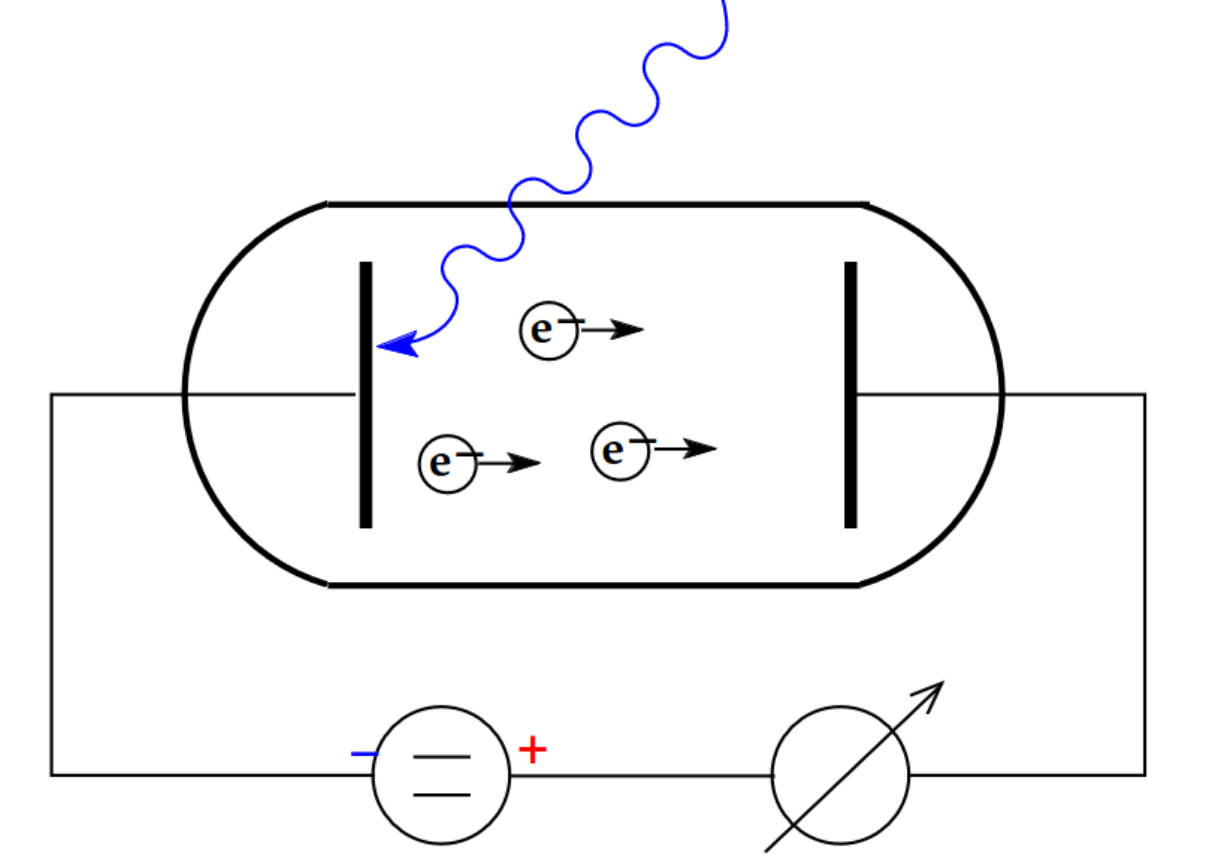
\includegraphics[width=0.8\textwidth]{content/Bilder/Schematischer_Aufbau.png}
  \caption{Schematische Darstellung des Fotoeffekts und einem Gegenfeld.}
  \label{fig:Schematische_Idee}
\end{figure}
Bei Durchführung der Bestrahlung der Metallplatte mit Licht werden 
verschiedene Eigenschaften ddes Fotoeffekts deutlich. 
Der Photostrom ist instantan mit der Bestrahlung des Metalls messbar.
Außerdem ist die Anzahl der ausgelösten Elektronen direkt proportional zur Lichtintensität 
bei einer festen Frequenz.
Zudem gibt es für jedes Material eine feste Grenzfrequenz, ab der Eletronen ausgelöste 
werden. Diese Grenzfrequenz ist unabhängig von der Lichtintensität. 
Die Energieverteilung der Elektronen hängt von der verwendeten Lichtfrequenz ab. 
Die klassische Interpretation des Lichts als elektromagnetische Welle 
kann allein die Eigenschaft erklären, dass die Anzahl der ausgelösten
Elektronen direkt proportionale zu der Intensität des einstrahlenden 
Lichtes abhängt. Daher müssen quantenmechanische Erklärungen verwendet werden. 
Ein wichtiger Faktor ist, dass die Elektronen im Material bereits eine 
bestimmte Energie besitzen, die durch die Fermi-Dirac Verteilung gegeben ist. 
Diese Verteilung ist in Abbildung (\ref{fig:Fermi_Dirac}) zu sehen. 
\begin{figure}[H]
    \centering
    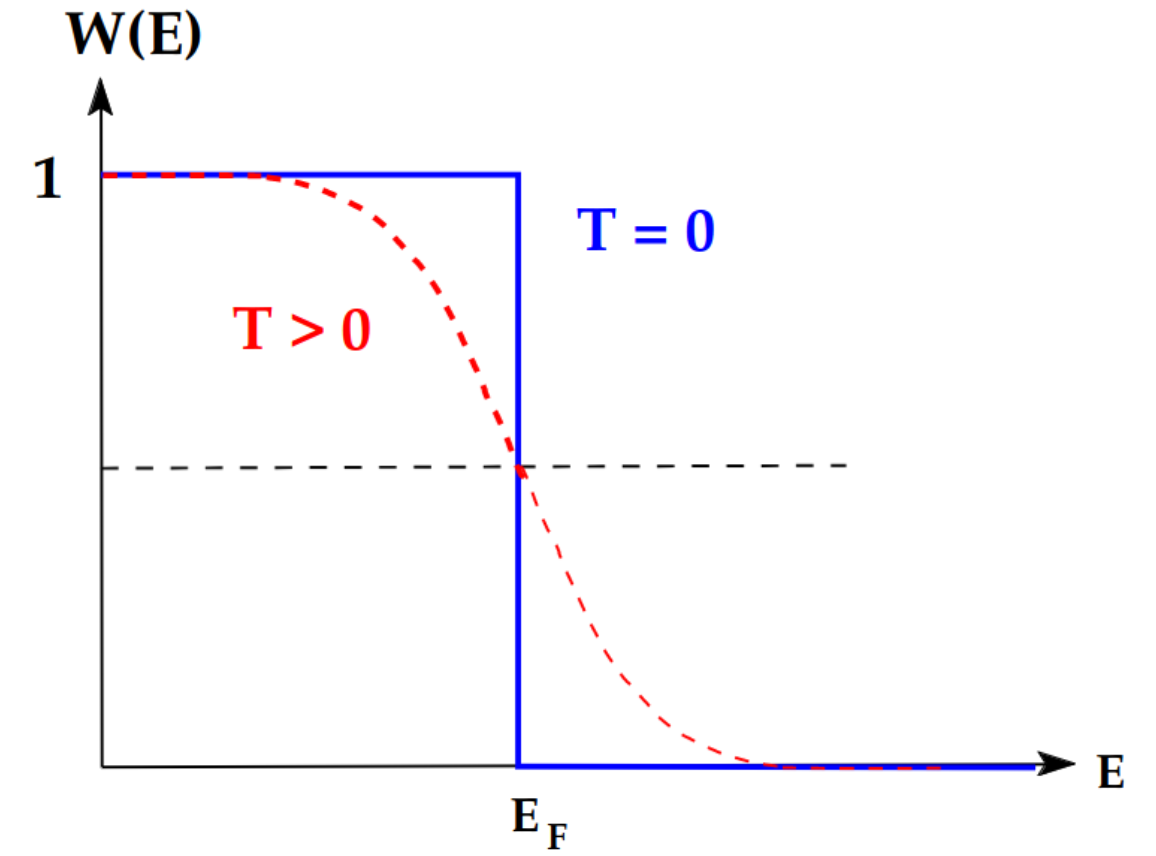
\includegraphics[width=0.7\textwidth]{content/Bilder/Fermi_Dirac.png}
    \caption{Wahrscheinlichkeit, dass ein Zustand mit bestimmter Energie im thermischen Gleichgewicht ist.}
    \label{fig:Fermi_Dirac}
  \end{figure}
\subsection{Vorbereitungsaufgaben}
\label{sec:Vorbereitungsaufgaben}
Zur Vorbereitung sollen die ausgetrahlten Wellenlängen einer Hg-Hochdrucklampe
recherchiert werden. Die Wellenlängen sind zusammen mit den entsprechenden Farben, Frequenzen und Energien in Tabelle 
(\ref{tab:Wellenlaengen}) aufgelistet. 
\begin{table}[H]
    \centering
    \caption{Von Hg-Lampe emittierte Wellenlängen mit Frequenz $\nu$ und Energie.}
    \label{tab:Wellenlaengen}
    \begin{tblr}{colspec={c c c c}}
        \toprule
        $\text{Farbe}$ & $\text{Wellenlänge} \left[\unit{\nano\meter}\right]$ & $\nu \left[\unit{\tera\hertz}\right]$ & $\text{Energie} \left[\unit{\eV}\right]$\\
        \midrule  
        \text{violett} & 404,66 & 740,85 & 3,06 \\
        \bottomrule
    \end{tblr}
\end{table}